\documentclass[]{article}
\usepackage{lmodern}
\usepackage{amssymb,amsmath}
\usepackage{ifxetex,ifluatex}
\usepackage{fixltx2e} % provides \textsubscript
\ifnum 0\ifxetex 1\fi\ifluatex 1\fi=0 % if pdftex
  \usepackage[T1]{fontenc}
  \usepackage[utf8]{inputenc}
\else % if luatex or xelatex
  \ifxetex
    \usepackage{mathspec}
  \else
    \usepackage{fontspec}
  \fi
  \defaultfontfeatures{Ligatures=TeX,Scale=MatchLowercase}
\fi
% use upquote if available, for straight quotes in verbatim environments
\IfFileExists{upquote.sty}{\usepackage{upquote}}{}
% use microtype if available
\IfFileExists{microtype.sty}{%
\usepackage{microtype}
\UseMicrotypeSet[protrusion]{basicmath} % disable protrusion for tt fonts
}{}
\usepackage[margin=1in]{geometry}
\usepackage{hyperref}
\hypersetup{unicode=true,
            pdfborder={0 0 0},
            breaklinks=true}
\urlstyle{same}  % don't use monospace font for urls
\usepackage{graphicx,grffile}
\makeatletter
\def\maxwidth{\ifdim\Gin@nat@width>\linewidth\linewidth\else\Gin@nat@width\fi}
\def\maxheight{\ifdim\Gin@nat@height>\textheight\textheight\else\Gin@nat@height\fi}
\makeatother
% Scale images if necessary, so that they will not overflow the page
% margins by default, and it is still possible to overwrite the defaults
% using explicit options in \includegraphics[width, height, ...]{}
\setkeys{Gin}{width=\maxwidth,height=\maxheight,keepaspectratio}
\IfFileExists{parskip.sty}{%
\usepackage{parskip}
}{% else
\setlength{\parindent}{0pt}
\setlength{\parskip}{6pt plus 2pt minus 1pt}
}
\setlength{\emergencystretch}{3em}  % prevent overfull lines
\providecommand{\tightlist}{%
  \setlength{\itemsep}{0pt}\setlength{\parskip}{0pt}}
\setcounter{secnumdepth}{5}
% Redefines (sub)paragraphs to behave more like sections
\ifx\paragraph\undefined\else
\let\oldparagraph\paragraph
\renewcommand{\paragraph}[1]{\oldparagraph{#1}\mbox{}}
\fi
\ifx\subparagraph\undefined\else
\let\oldsubparagraph\subparagraph
\renewcommand{\subparagraph}[1]{\oldsubparagraph{#1}\mbox{}}
\fi

%%% Use protect on footnotes to avoid problems with footnotes in titles
\let\rmarkdownfootnote\footnote%
\def\footnote{\protect\rmarkdownfootnote}

%%% Change title format to be more compact
\usepackage{titling}

% Create subtitle command for use in maketitle
\providecommand{\subtitle}[1]{
  \posttitle{
    \begin{center}\large#1\end{center}
    }
}

\setlength{\droptitle}{-2em}

  \title{}
    \pretitle{\vspace{\droptitle}}
  \posttitle{}
    \author{}
    \preauthor{}\postauthor{}
    \date{}
    \predate{}\postdate{}


\begin{document}

\hypertarget{the-telemarketer-model}{%
\section{THE TELEMARKETER MODEL}\label{the-telemarketer-model}}

This model was produced by S. Railsback and V. Grimm for the book:
\emph{Agent-based and Individual-Based Modeling: A Practical
Introduction}, 2nd edition (2019).

This version is the first, basic version of the model as described in
Section 13.3.1.

Let us visit the formerly remote land of Wasellya, which has developed
very rapidly, so suddenly all its citizens have telephones. Naturally,
the ``invasion'' of telephone technology is followed rapidly by an
invasion of people tempted to start a telemarketing business. Is this a
good business risk? How many telemarketers will stay in business, for
how long? How does the average life span of a telemarketing company
depend on how many are started? Here is the ODD description of a simple
model for this problem; you should implement the model.

\hypertarget{overview}{%
\subsection{OVERVIEW}\label{overview}}

\hypertarget{purpose-and-patterns}{%
\subsubsection{PURPOSE AND PATTERNS}\label{purpose-and-patterns}}

The real purpose of this model is to illustrate several kinds of
interaction: how to model them and what their effects are on system
behavior. While the modeled system is imaginary and none too serious, it
does represent a common ABM scenario: a system of agents that compete
for a resource and grow or fail as a result. For such a model we define
only simple, general patterns as the criteria for its usefulness: two
measures of system performance---the changes over time in the number of
telemarketers in business and the median time that telemarketers stay in
business---depend on how many agents there are and how they interact.

\hypertarget{state-variables-and-scales}{%
\subsubsection{STATE VARIABLES AND
SCALES}\label{state-variables-and-scales}}

This model has two kinds of entities: potential customers (households
with telephones), which we represent as patches, and telemarketers,
which are turtles. The model is spatial: we represent the territory over
which a telemarketer contacts potential customers, and the distance
between telemarketers and potential customers, in arbitrary units equal
to one patch size. World wrapping is turned off, so the space does have
borders.

Potential customers have only one state variable in addition to their
location. This is a boolean variable that represents whether they have
been called by a telemarketer during the current time step. (In the
NetLogo program, you can use the patch's color for this variable: the
patch is one color if it has not yet been called, and a second color if
it has been called.)

The telemarketers have state variables for their (floating point)
location in space, and for size, which represents how many staff,
dialing machines, telephone lines, and other resources they have.
Telemarketers also have a state variable for their bank balance, the
amount of money they have to pay expenses and grow.

The model runs at a weekly time step. Simulations are 200 time steps
long. There are 40,401 potential customers (the patches in a NetLogo
world with the origin in the middle and maximum \emph{x-} and \emph{y-}
coordinates of 100).

\hypertarget{process-overview-and-scheduling}{%
\subsubsection{PROCESS OVERVIEW AND
SCHEDULING}\label{process-overview-and-scheduling}}

The model includes four actions executed in the following order each
time step.

First, the patches all reset their state variable for whether they have
been called by a telemarketer this week to ``no'' (i.e., set pcolor to
the color representing ``not called yet'').

Second, the telemarketers do their sales calls, using the submodel
detailed below. Each marketer makes all its calls before the next
marketer does its calls. A telemarketer calls a number of potential
customers; this number increases with telemarketer size. The potential
customers are within a radius of the telemarketer that increases with
the marketer's size. (In this early stage of Wasellya's development, the
cost of phone calls increases steeply with their distance.) Each
potential customer buys something from the telemarketer if it has not
been called previously in the time step, then sets its variable for
whether it has been called to ``yes'' (i.e., changes its pcolor). If
that variable was already ``yes,'' the potential customer hangs up on
the telemarketer and buys nothing. (Wasellyans are not very
sophisticated yet, but they have short tempers.) The order in which the
telemarketers carry out this second action is obviously important
because the first marketer to call a customer makes a sale, whereas
marketers who call the same customer later in the week make no sale. We
will explore this issue in chapter 14, but here we use NetLogo's default
scheduling, which is that the order in which telemarketers execute the
action is randomly shuffled each time step.

Third, the telemarketers do their weekly accounting; the submodel is
fully described below at item 7. Income is determined from the number of
successful calls. Costs of business increase linearly with size. The
bank balance state variable is updated by adding sales income and
subtracting costs. If the bank balance is negative, the telemarketer
goes out of business and is removed from the model. The telemarketer
increases its size if its bank balance is high enough.

The fourth action is observer updates: outputs such as the number of
telemarketers still in business, a histogram of their size, and the
total number of sales, are reported.

\hypertarget{design-concepts}{%
\subsection{DESIGN CONCEPTS}\label{design-concepts}}

\emph{Basic principles.} The basic concept explored in this model is
competition among agents for resources that are limited but renewed.

\emph{Emergence.} The primary model results we are interested in are
patterns in the number of telemarketers in business over time as a
simulation proceeds. (The size distribution of telemarketing
companies---how many big ones and how many small ones there are, over
time---is another potentially interesting result.) These results emerge
from how many telemarketers are initialized, how they compete with each
other, how many customers there are and how they respond to calls, and
how the telemarketers turn their income into growth.

\emph{Adaptive behavior.} The telemarketers adapt to their sales success
by deciding whether to grow in size, and how much to grow. However, this
behavior is modeled very simply and rigidly: any bank balance above a
minimum is automatically spent to increase the company's size. Potential
customers have one simple behavior: when called, they decide whether to
make a purchase by whether they have already been called during the time
step. There are no adaptive tradeoff decisions.

\emph{Prediction.} The telemarketer's adaptive behavior is based on an
implicit prediction that if sales are higher than needed to maintain a
minimum bank balance, then increasing in size will further increase
income. (Note that this implicit prediction is different from---and
perhaps not as smart as---predicting that growth will be beneficial as
long as income is increasing. Is it smart to grow when income is high
but decreasing?)

\emph{Sensing.} The telemarketers sense whether each potential customer
has already bought something on the current time step.

\emph{Interaction.} There are two kinds of interaction: between
telemarketers and potential customers, and among the telemarketers. The
telemarketers interact directly with potential customers by
communicating to find out whether the customers will buy, and then by
making the customers change their state to indicate that they bought
during the current time step. The telemarketers' interactions with each
other are mediated by the resource they compete for: customers. When the
territories of telemarketers overlap, customers of one telemarketer are
no longer available as potential sales for other telemarketers.

\emph{Stochasticity.} There are three stochastic elements of the model.
First, telemarketers are placed at random locations when the model is
initialized. Second, telemarketers select the customers they call
randomly from all the potential customers (see the telemarketer sales
submodel, below). Third, the order in which telemarketers make their
calls is randomly shuffled each time step, to avoid bias from the
advantage that first callers have.

\emph{Observation.} The primary outputs of interest can be observed via
a plot of the number of telemarketers still in business. However, to
understand how the system is working it is also useful to have a
histogram of telemarketer sizes (figure 13.1). The number of
telemarketers in business is output to a file each time step so that
statistics on how long telemarketers stay in business (e.g., their
median life span---the time at which half have failed) can be calculated
at the end of a simulation.

\begin{figure}
\centering
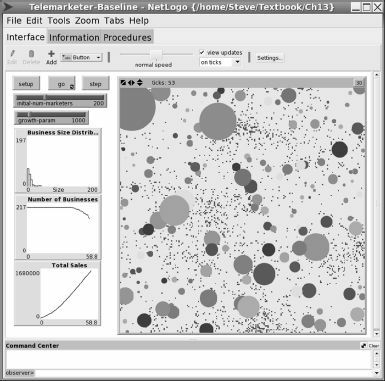
\includegraphics{fig_13_1.jpg}
\caption{Fig. 13.1}
\end{figure}

\hypertarget{details}{%
\subsection{DETAILS}\label{details}}

\hypertarget{initialization}{%
\subsubsection{INITIALIZATION}\label{initialization}}

The model is initialized with 200 telemarketers, each with size 1.0 and
bank balance of 0.0, and a location chosen randomly from all the points
in the space, with equal probability for all points. (For display, these
are given random colors and drawn as circles.) The potential customers
have their variable for whether they have been called during the week
initialized to "no.

\hypertarget{input-data}{%
\subsubsection{INPUT DATA}\label{input-data}}

This model uses no time-series inputs.

\hypertarget{submodels}{%
\subsubsection{SUBMODELS}\label{submodels}}

\emph{Telemarketer sales.} A telemarketer's potential customers are the
patches within the marketer's territory, which is a circle around the
marketer's location with radius equal to 10 times the square root of the
telemarketer's size. The maximum number of calls a telemarketer can make
each step is 100 times its size. (Therefore, unless the territory
overlaps the space's edge, there are about 3.14 times more potential
customers than calls.) If the number of potential customers is greater
than the maximum number of calls, then the telemarketer randomly chooses
this maximum number of potential customers to call. If instead the
number of potential customers is less than the maximum number of calls
(possible for marketers on the edge of the space), then all potential
customers are called. The number of successful sales is the number of
potential customers called who have not previously been called by a
different telemarketer on the same time step (i.e., they still were the
color representing ``not called yet''). (Programming hint: It is not
necessary to simulate each sales call! Telemarketers can simply identify
a subset of potential customers that they sell to, count that subset,
and then ask its members to identify themselves as having been called.)

\emph{Telemarketer accounting.} The weekly cost of business is equal to
the telemarketer's size times 50. (Money units are arbitrary.) The
income from sales is 2 times the number of successful sales. The bank
balance is updated by adding the income from sales and subtracting the
cost of business.

A parameter growth-param determines how rapidly telemarketer businesses
grow. If the new bank balance is greater than growth-param, then the
telemarketer converts all but growthparam of this balance to increase in
growth. For every 1 unit of bank balance above growthparam, the
telemarketer's size increases by the amount of a parameter
money-size-ratio, which is 0.001. The value of growth-param is 1000, so,
for example, if the new bank balance is 1500, then bank balance is set
to 1000 and the telemarketer's size increases by 0.5 (which is $[1500 -
1000] \times 0.001$). (Telemarketer size never decreases.)

If the new bank balance is less than zero, the telemarketer goes out of
business and is removed from the model immediately.


\end{document}
